\subsection{System components}
The proposed system consists of several components that interact together. To satisfy the non-functional requirement PT-NFR-1, we design the architecture of our system as presented in \ref{fig:arch-ver2} (p. \pageref{fig:arch-ver2}). The main point of user interaction for both primary user and secondary user is the system front end. The front end communicates with Ethereum blockchain via Ethereum node, to deploy a custom smart contract, which operates logic described in figure \ref{fig:simple-logic} (p. \pageref{fig:simple-logic}) and with a back end acts as a communication channel\footnotemark between users. To operate its logic, the smart contract communicates with an oracle. The oracle queries a blockchain explorer provider to learn about the status of a transaction and sends the updates back to the smart contract. User triggers the events in the Android application and validates events on the blockchain. The validation should be done with use of other systems than the Android application itself. Figure \ref{fig:system-overview} depicts the system parts and their relations.

\footnotetext{In the previous examples, we have always considered that the two trading parties -- Alice and Bob agreed on the terms of the transaction beforehand using a separate channel. For this prototype, we have decided to include a communication channel, to enable users interact and agree on the transaction terms within the prototype. While this functionality is certainly not novel, nor it is the focus of this project, it complements the prototype and showcases, how it could be used in real-world.}

\begin{figure}[p]
    \centering
    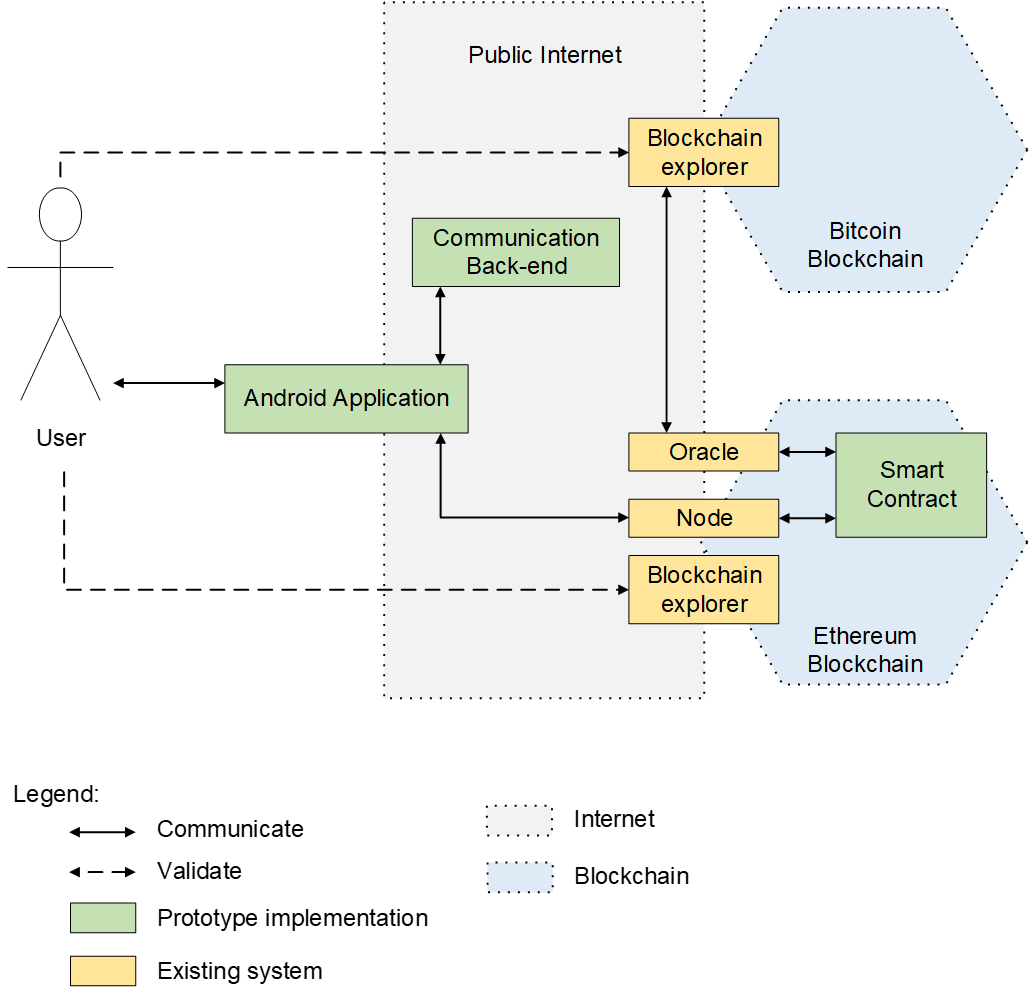
\includegraphics[width=\textwidth]{system-overview}
    \caption[itemize]{
    Overview of the system parts:
    \begin{enumerate*}[label=(\roman*)]
        \item \textit{User} communicates directly with the Android application and verifies data on the blockchain.
        \item \textit{Android application} fetches data about existing offers from the communication back-end and sends new smart contracts to the Ethereum node.
        \item \textit{Node} communicates with other nodes in the Ethereum network, maintains the status of the blockchain and deploys new smart contracts to the network.
        \item \textit{Smart contract} contacts oracle after deployment and holds the funds until the oracle has cleared the transaction as approved.
        \item The \textit{oracle} queries the Bitcoin block explorer to learn about the status of the transaction and communicates the result back to the smart contract.
        \item \textit{Communication back end} communicates only with the Android application. It holds details about users' offers and supports the trading interaction between users.
    \end{enumerate*}}
    \label{fig:system-overview}
\end{figure}